\section{Implementation}
\subsection{Modules}
The following modules have been defined:
\begin{itemize}
	\item \textbf{Transmitter}: duty of sending a packet to a specific channel. Computes \textbf{mean buffer size} statistic.% Parameters: $lambda$, $p$, packetsInQueue Signal (for the queue)
	\item \textbf{Channel}: duty of checking every channel in each timeslot for any collision. Computes \textbf{throughput}, \textbf{collision count} and \textbf{response time} (generalized for all receivers) statistic.% Parameters: $T_{timeslot}$, Throughput Signal
	\item \textbf{Receiver}: duty of receiving a packet from the channel. Computes \textbf{response time} statistic.
\end{itemize}

\begin{figure}[H]
	\centering
	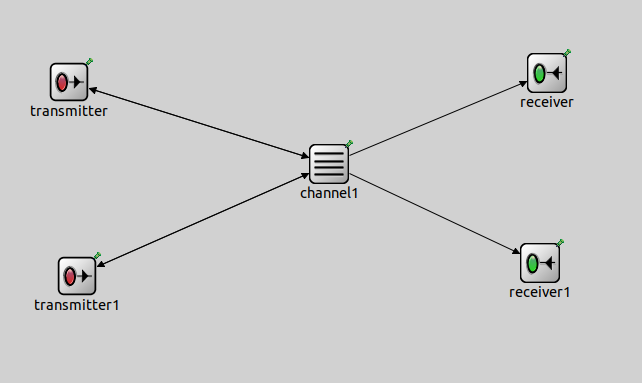
\includegraphics[width=0.6\textwidth]{img/network.png}
	\caption{Network example}
	\label {img: network}
\end{figure}

\subsection{Messages}
A new format of message has been defined, in order to store all packet information, with the following fields:
\begin{itemize}
	\item \textit{simtime$\_$t creationTime}: time in which the packet arrives for the first time at the \textbf{Transmitter}
	\item \textit{int idChannel}: \textbf{Channel} chosen for the current transmission, may change in case of collision
	\item \textit{int idTransmitter}: Id of the module \textbf{Transmitter} that has sent the message
	\item \textit{int idGate}: Id of the gate in which the \textbf{Transmitter} is linked to the \textbf{Channel}
\end{itemize}

\subsection{Modules Behaviour}
\subsubsection{\textit{Transmitter} Module Behaviour in the implementation}
\begin{enumerate}
	\item Message arrival at the \textit{Transmitter}:
	\begin{itemize}
		\item \textbf{IF} an \textit{ACK} has been received, the packet at the top of the queue can be removed. \textbf{GOTO (2)}
		\item \textbf{ELSE IF} a \textit{NACK} has been received, then the \textit{Transmitter} starts his backoff time and \textbf{waits for another message}.
		\item \textbf{ELSE IF} a \textit{Synchronization message} has been received \textbf{AND} the \textit{Transmitter} is not in backoff-time \textbf{GOTO (2)}
		\item \textbf{ELSE IF} a \textit{packet} arrives at the \textit{Transmitter}, the \textit{Transmitter} stores the packet in the queue, make a reschedule of the arrival of the next packet and \textbf{waits for another message}
	\end{itemize}
	\item The \textit{Transmitter} tries to send the packet
	\begin{itemize}
		\item \textbf{IF} success on the Bernoullian Experiment, then the packet will be forwarded to the \textit{Channel}.
		\item \textbf{ELSE waits for another message}
	\end{itemize}
\end{enumerate}
\subsubsection{\textit{Channel} Module Behaviour in the implementation}
\begin{enumerate}
	\item The \textit{Channel} wakes up at the beginning of each time slot and checks his channels status.
	\begin{itemize}
		\item \textbf{IF} two or more packets have arrived in the same channel, the \textit{Channel} will send a NACK to the \textit{Transmitters} that have forwarded the packets in that specific channel.
		\item \textbf{ELSE IF} one and only one packet has arrived in a channel, the \textit{Channel} will send an ACK to the relative \textit{Transmitter} and will forward the packet to the \textit{Receiver}.
		\item \textbf{ELSE} the \textit{Transmitters} that did not send a packet will receive from the Channel a \textit{Synchronization Message}
	\end{itemize}
	\item The \textit{Channel} will gather of the packets for the current time slot, to be processed in the next one. So this means that if the channel receives packets in time-slot \emph{j}, then the information about collisions are provided to transmitters in time-slot \emph{j+1}. Hence, from the point of view of the transmitter, the information received at \emph{j+1} are referred to events took place in \emph{j}.
\end{enumerate}
\subsubsection{\textit{Receiver} Module Behaviour in the implementation:}
\begin{enumerate}
	\item The \textit{Receiver} wakes up when a packet arrives. Due to the fact that the receiver essentially has the only duty of receiving packets. It computes statistics on the number of packets received mainly for debugging purpose.
\end{enumerate}